\chapter{Результаты исследования и сравнительный анализ} \label{ch4}


% не рекомендуется использовать отдельную section <<введение>> после лета 2020 года
%\section{Введение} \label{ch4:intro}


	
\section{Результат првоерки статистической гипотезы} \label{ch4:sec1}
Критерий Вилконсона показал следующие результаты:\\

Пять изображений \textbf{модельной} мушки: согласно критерию изменение среднеквадратичных отклонений значений интенсивностей пикселей до и после применения инструмента удаления автофлуоресценции AFid \underline{статистически значимо} при $\alpha = 0.5$ для вариации алгоритма с автоматическим определением оптимального числа кластеров (3 вариант, см. \ref{variations}) и вариации с межканальным пороговым значений коэффициентов корреляции Пирсона (1 вариант, см. \ref{variations}). А значит можно утверждать, что для двух вариаций алгоритма AFid действительно паразитное свечение удаляется.

Для вариации с числом кластеров равным шести (2 вариант, см. \ref{variations}), согласно критерию гипотеза принимается только для первого канала. Для изображений M4, M6, M7 второго канала изменений среднеквадратичных отклонений нет. А значит свечение не удалилось.


Четыре изображения мушки \textbf{дикой породы} Sz-139: для вариации с числом кластеров равным шести в изменение среднеквадратичных отклонений значений интенсивностей пикселей до и после применения AFid статистически значимой разницы также нет.

Вариации алгоритма с автоматическим определением оптимального числа кластеров и с межканальным пороговым значений коэффициентов корреляции Пирсона согласно критерию Вилконсона удаляют паразитное свечение при уровне значимости 7\%. То есть в отличие от модельной мушки - для дикой породы в изменении среднеквадратичных отклонений \underline{статистическая значимость более слабая} (на уровне меньше 10\%) 

$\alpha$ - уровень значимости.

%\begin{table} [htbp]% Пример оформления таблицы
%	\centering\small
%	\caption{Пример представления данных для сквозного примера по ВКР \cite{Peskov2004}}%
%	\label{tab:ToyCompare}		
%		\begin{tabular}{|l|l|l|l|l|l|}
%			\hline
%			$G$&$m_1$&$m_2$&$m_3$&$m_4$&$K$\\
%			\hline
%			$g_1$&0&1&1&0&1\\ \hline
%			$g_2$&1&2&0&1&1\\ \hline
%			$g_3$&0&1&0&1&1\\ \hline
%			$g_4$&1&2&1&0&2\\ \hline
%			$g_5$&1&1&0&1&2\\ \hline
%			$g_6$&1&1&1&2&2\\ \hline		
%		\end{tabular}
%%	\caption*{\raggedright\hspace*{2.5em} Составлено (или/и рассчитано) по \cite{Peskov2004}} %Если проведена авторская обработка или расчеты по какому-либо источнику	
%	\normalsize% возвращаем шрифт к нормальному
%\end{table}


\section{Результаты кластеризации и фильтрации} \label{ch4:sec2}

\subsection{Результат фильтрации}
Ниже приведены построенные гистограммы для удалени шума изображения модельной мушки M4.

\begin{figure}[H]
	\centering
	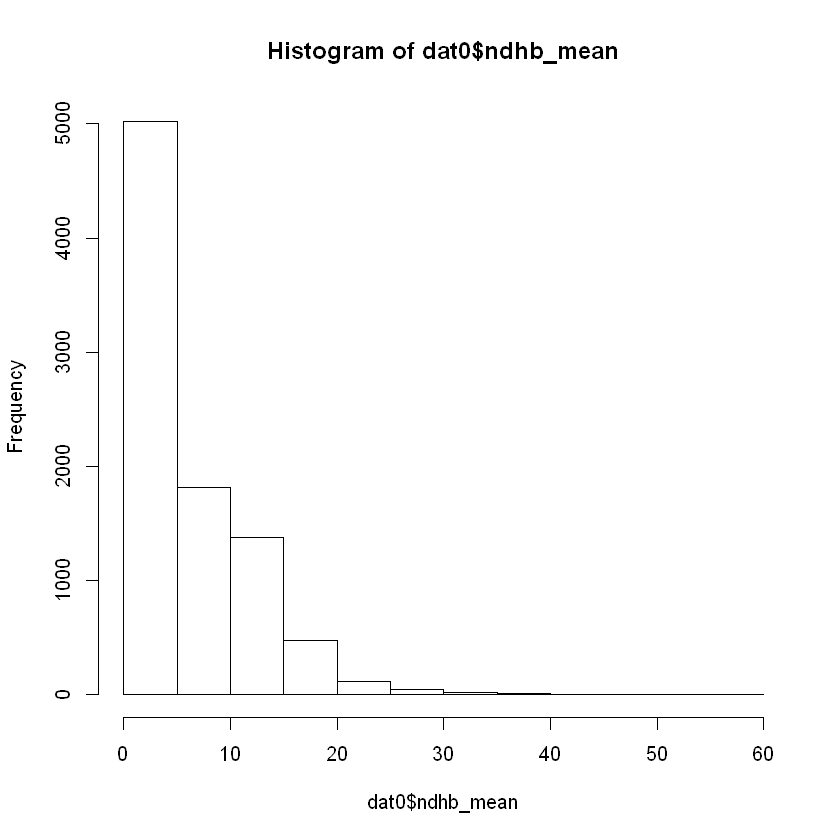
\includegraphics[width=7cm, height=7cm]{hist_m4_1}
	\caption{Гистограмма частоты встречаемости пикселей по мере увеличения значения интенсивности для изображения М4.}
	\label{hist_m4_1}
\end{figure}

\begin{figure}[H]
	\centering
	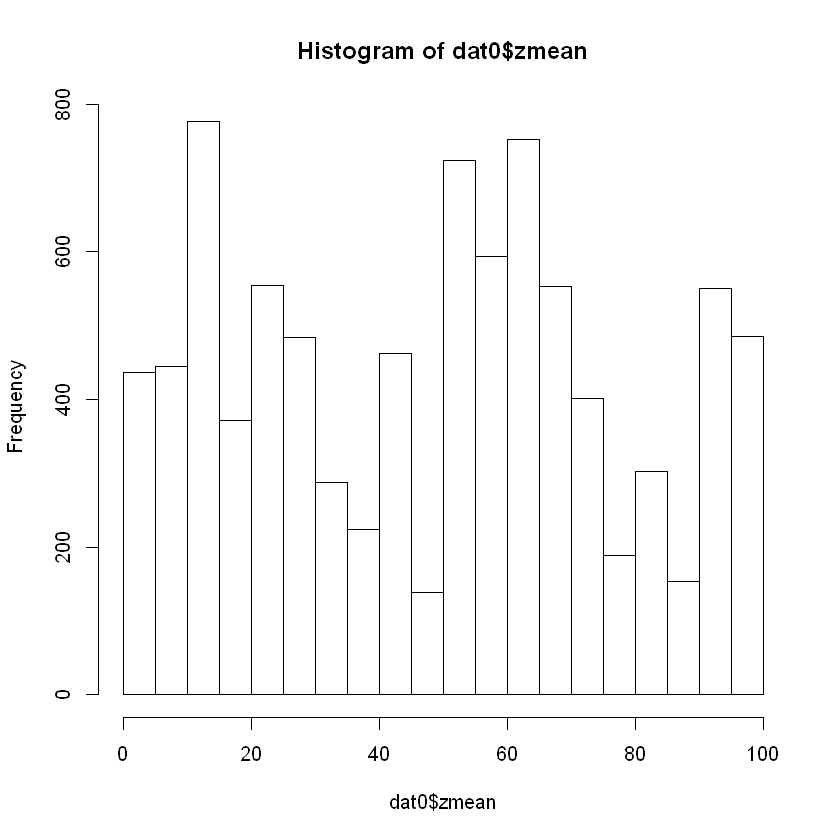
\includegraphics[width=7cm, height=7cm]{hist_m4_2}
	\caption{Гистограммма показывающая количество комплексов молекул для каждого слоя изображения М4.}
	\label{hist_m4_2}
\end{figure}

После удаления объектов подозрительных на шум (крайние объекты во второй гистограмме и имеющие очень малую интенсивность в первой) были получены следующие результаты фильтрации.


\begin{figure}[H]
	\centering
	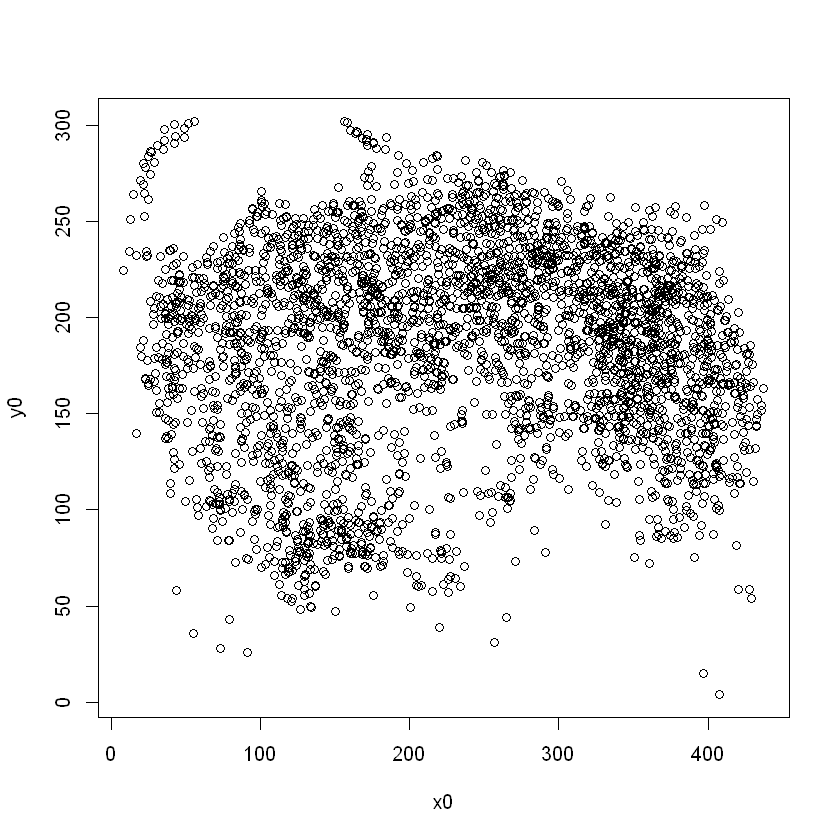
\includegraphics[width=7cm, height=7cm]{filt_m4_or}
	\caption{Результат фильтрации для изображения мозга модельной мушки М4.}
	\label{filt_m4_or}
\end{figure}


\begin{figure}[H]
	\centering
	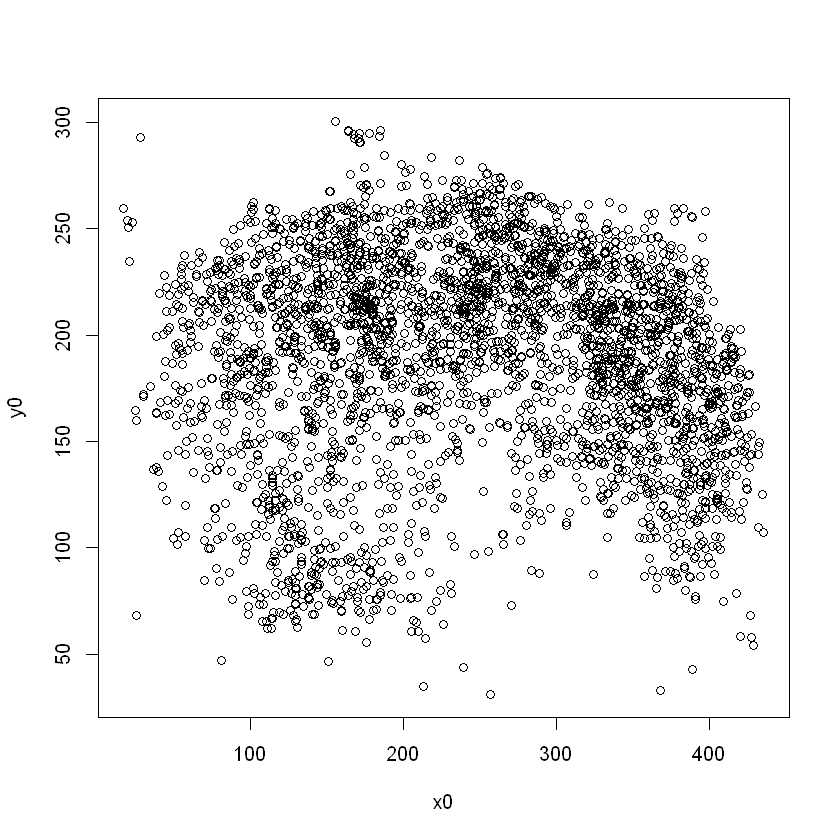
\includegraphics[width=7cm, height=7cm]{filt_m4_af}
	\caption{Результат фильтрации для изображения мозга модельной мушки М4 после применения инструмента удаления автофлуоресценции AFid.}
	\label{filt_m4_af}
\end{figure}


По результатам фильтрации можно сказать что после применения AFid изображение мозга лучше кластеризуется. Так, например, на рисунке \ref{filt_m4_af} убраны висячие артефакты которые присутствуют в изображении до применения AFid на рисунке \ref{filt_m4_or}.\\

(ДОПОЛНИТЬ ПОСЛЕ ВСЕХ РЕЗУЛЬТАТОВ)

%\FloatBarrier % заставить рисунки и другие подвижные (float) элементы остановиться



%% Вспомогательные команды - Additional commands
%
%\newpage % принудительное начало с новой страницы, использовать только в конце раздела
%\clearpage % осуществляется пакетом <<placeins>> в пределах секций
%\newpage\leavevmode\thispagestyle{empty}\newpage % 100 % начало новой страницы